\documentclass{article}

	\usepackage[english]{babel}
	\usepackage[T1]{fontenc}
	\usepackage{xspace}
	\usepackage{graphicx}
	\usepackage[export]{adjustbox}
	\usepackage[hidelinks,colorlinks=true,urlcolor=blue,linkcolor=black]{hyperref}
	\usepackage{microtype}

	\newcommand{\latex}{\LaTeX\xspace}
	\newcommand{\email}[1]{\texttt{#1}}
	\newcommand{\icon}[2]{\includegraphics[scale=#2]{../resources/#1}\xspace}

\begin{document}

\title{
	\icon{vscode_icon.png}{0.05}\\
	A Guide to \latex Editing in Visual Studio Code\\
	\large Written in \latex with Visual Studio Code
}
\author{
	Dan Arad\\
	\email{arda@post.bgu.ac.il}
}
\maketitle

\section{Introduction} \label{sec:introduction}
This guide's purpose is to help setup a comfortable and efficient workspace of \latex documents using \href{https://code.visualstudio.com/}{Visual Studio Code} (also known as VSCode). This also includes the ability to easily work with git version control, and keep generated files out of the way.\\
VSCode is a free open source powerful light-weight editor developed and maintained by Microsoft. The editor boasts many extensions and built-in git support, and is widely used. Among its many extensions, there is one called \href{https://marketplace.visualstudio.com/items?itemName=James-Yu.latex-workshop}{\latex Workshop}.\\
To me VSCode is the first choice for editing any kind of code, and for that reason I chose to see how well it will preform as a \latex editor. I was not dissapointed with the result.


\section{Basic Setup} \label{sec:basic_setup}
For the basic setup of VSCode with \latex I used \href{https://dev.to/nickymarino/lets-use-latex}{Nicky Marino's guide}, and this entire section is based on it.\\
At the conclusion of this basic setup, you will have everything you need to get going:
\begin{itemize}
	\item{Syntax highlighting for \latex with basic auto-completion}
	\item{Preview option that is updated either manualy or on save}
	\item{An outline of your \latex document}
	\item{Error and warning pane}
\end{itemize}
Figure \ref{fig:vscode_with_latex_highlights} displays the outcome and the different components.\\
\begin{figure}
	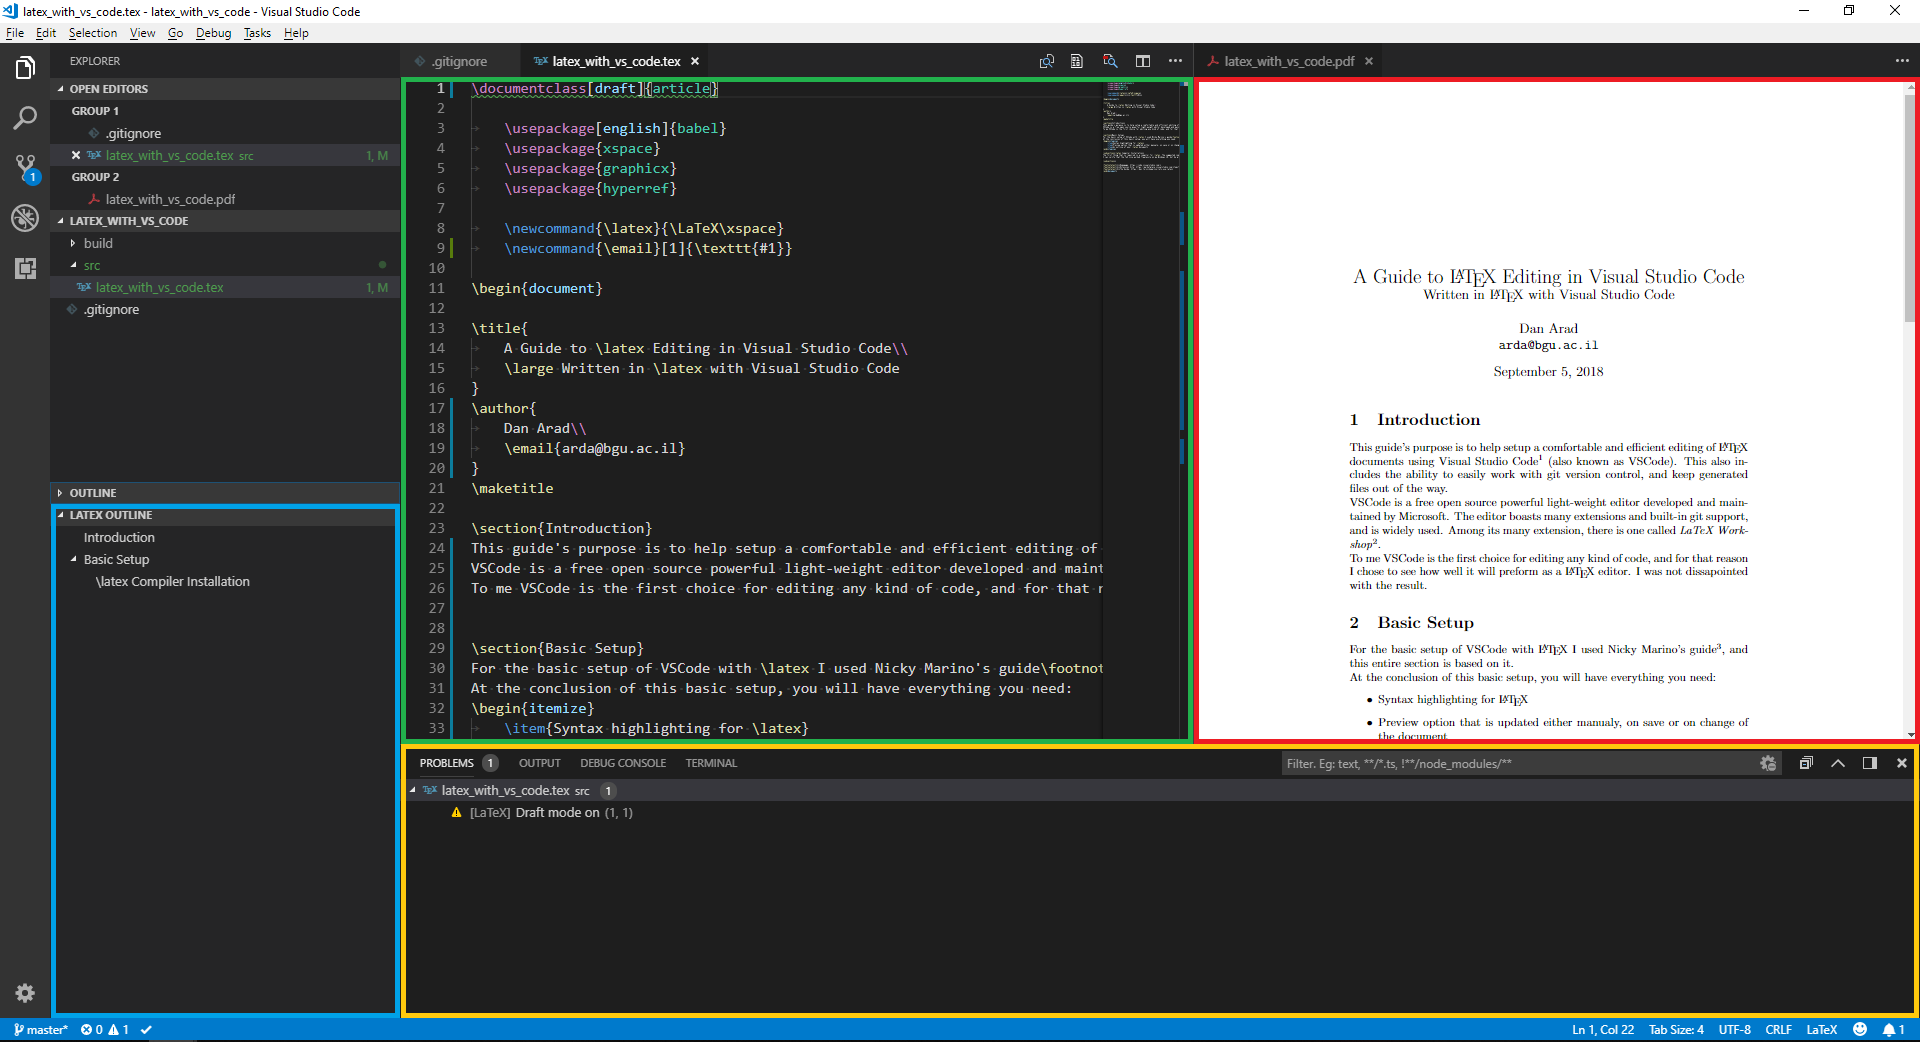
\includegraphics[width=\linewidth]{../resources/vscode_with_latex_highlights.png}
	\caption{Green: Code Highlighting, Red: Preview, Blue: Outline, Yellow: Errors and Warnings}
	\label{fig:vscode_with_latex_highlights}
\end{figure}
\textbf{Note:} As of version 5.9.0 of \latex Workshop, the layout has become part of the left pane displays, and can be accessed by pressing the \icon{tex_icon.png}{0.3} icon.

\subsection{\latex Compiler Installation}
The first thing that is required is a compiler for \latex. The suggested compiler is \href{https://www.tug.org/texlive/}{TeX Live} for Windows and Linux, and \href{https://www.tug.org/mactex/}{MacTex} for MacOS.\\
I can verify that the \emph{TeX Live} worked flawlessly on my Windows 10, but be prepared - It's a very long installation.

\subsection{VScode and \latex Workshop Installation}
If you don't have VSCode installed, install it from the official website.\\
Then, in VSCode go to the extension marketplace by clicking the \icon{extensions_icon.png}{0.4} button in the leftmost pane, or by using the shortcut \texttt{Ctrl+Shift+X}. Search for \latex Workshop, click install, and when finished, click reload.\\
After the editor reloads, you should be able to use all of the previously discussed functionalities.


\section{Additional Know-How} \label{sec:additional_know_how}
I will not go in depth explaining the features of VSCode, but I do find it important to talk about the issue of extension commands and settings.

\subsection{Commands}
In VSCode, each extension may define commands that can be run by the user. To run a command use the \texttt{Ctrl+Shift+P} shortcut that opens a context menu with all available commands, as shown in figure \ref{fig:command_menu}.\\
\latex Workshop defines several such commands. The most useful I found are \emph{LaTeX Workshop: Build LaTeX project}, which can also be activated using \texttt{Ctrl+Alt+B}, \emph{laTeX Workshop: Clean up auxiliary files} and \emph{LaTeX Workshop: View LaTeX PDF file in VSCode tab}, that can also be triggered by using the \icon{preview_icon.png}{0.5} button that is located in the tabs area.
\begin{figure}
	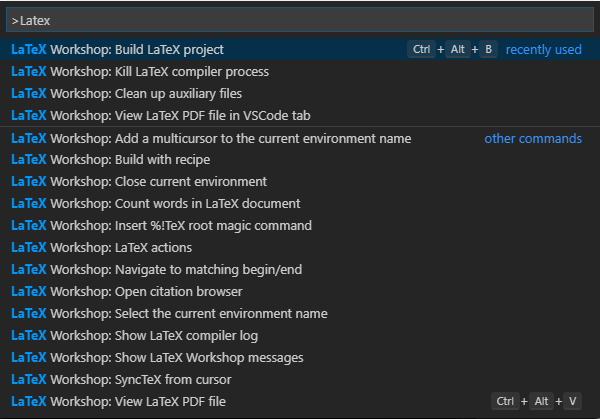
\includegraphics[width=\linewidth]{../resources/command_menu.png}
	\caption{The commands context menu}
	\label{fig:command_menu}
\end{figure}

\subsection{Settings}
Each extension also has its own settings that are controlled through the settings window of VSCode. The settings are grouped by category, and each extension has its own group.\\
To open the settings window go to \texttt{File -> Preferences -> Settings}, or use the \texttt{Ctrl+,} shortcut.\\
As can be seen in figure \ref{fig:settings_window}, The settings menu is split into two panes. The left pane shows all settings in their default values, while the right pane shows user (or workspace) settings that differ from the default.\\
\latex Workshop has a lot of configuration options, but it will work just fine left untouched. We will discuss some changes to the configuration in section \ref{sec:seperating_sources_from_outputs}.\\
\begin{figure}
	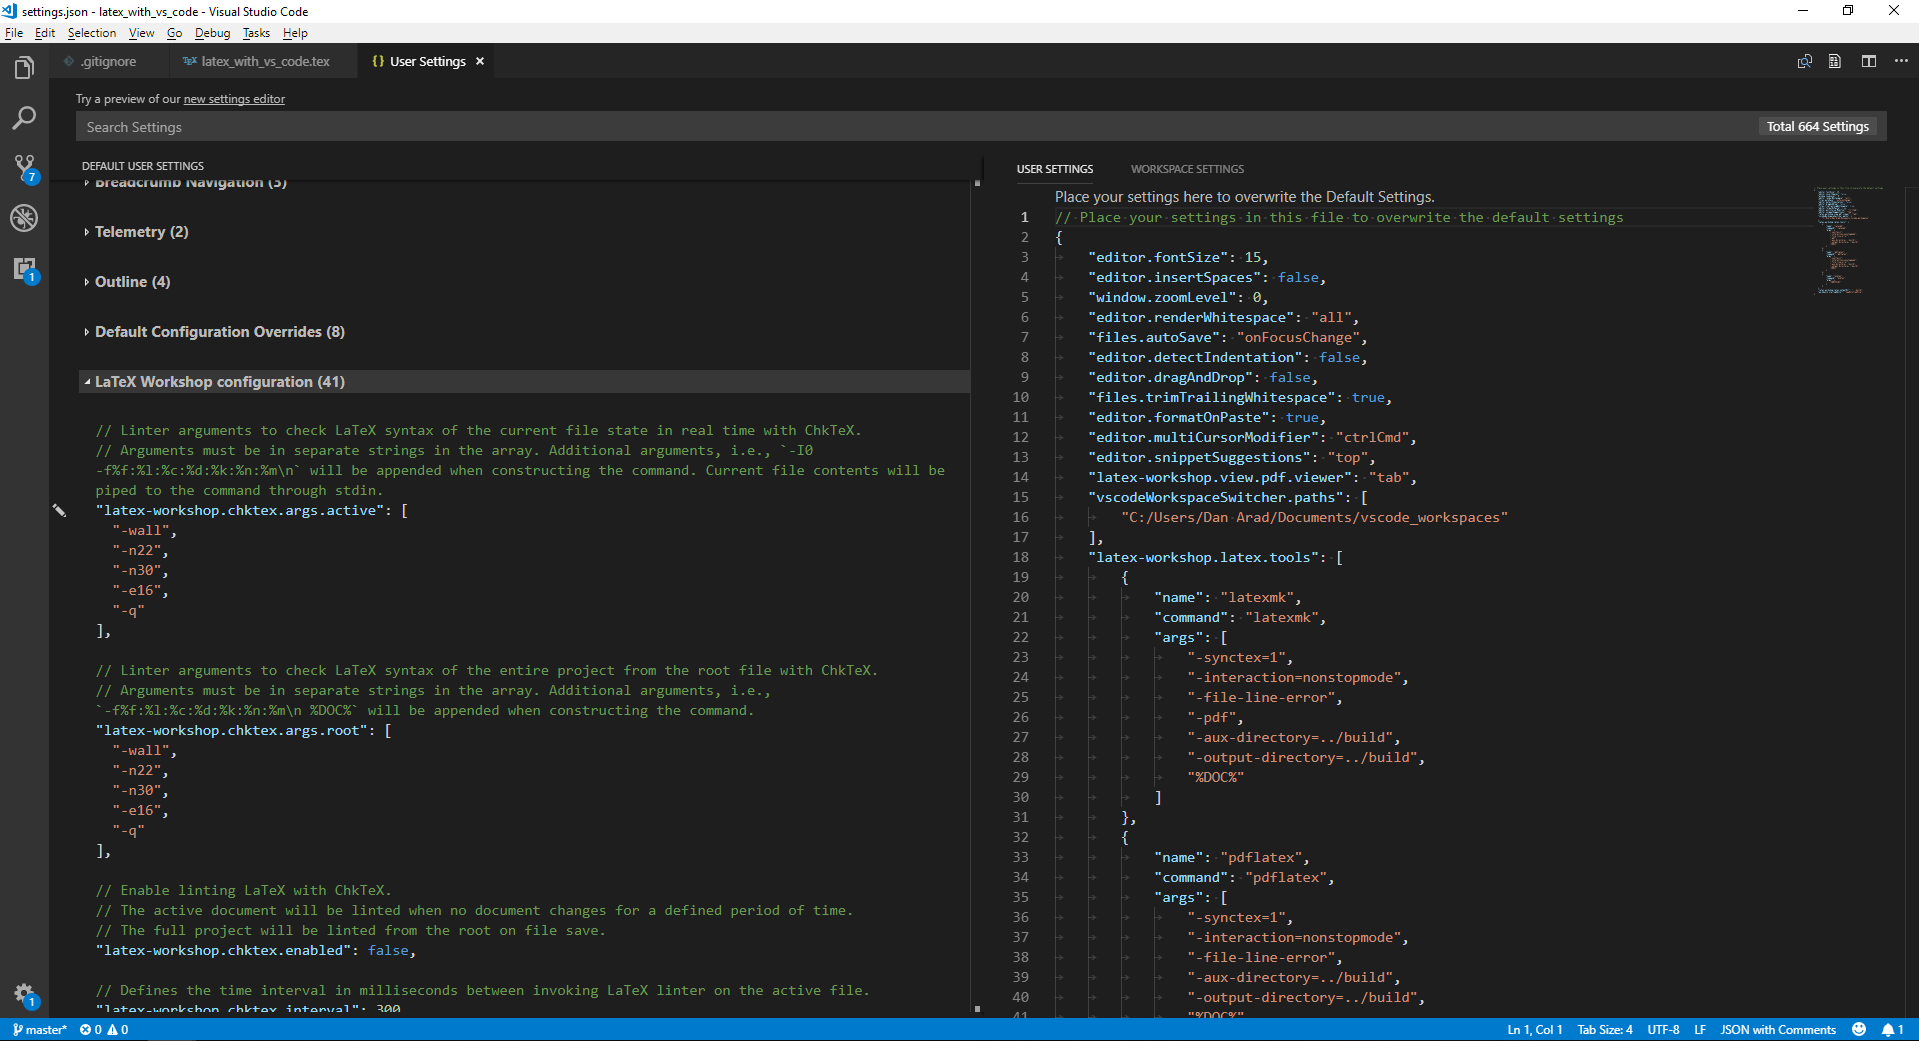
\includegraphics[width=\linewidth]{../resources/settings_window.png}
	\caption{The settings window with a view of the \latex Workshop settings}
	\label{fig:settings_window}
\end{figure}
\textbf{Note:} As of version 1.27 of VSCode, the settings interface has been changed, and is now more graphic. In order to get to the json based preview, use the menu as displayed in figure \ref{fig:v1_27_settings}.
\begin{figure}[h!]
	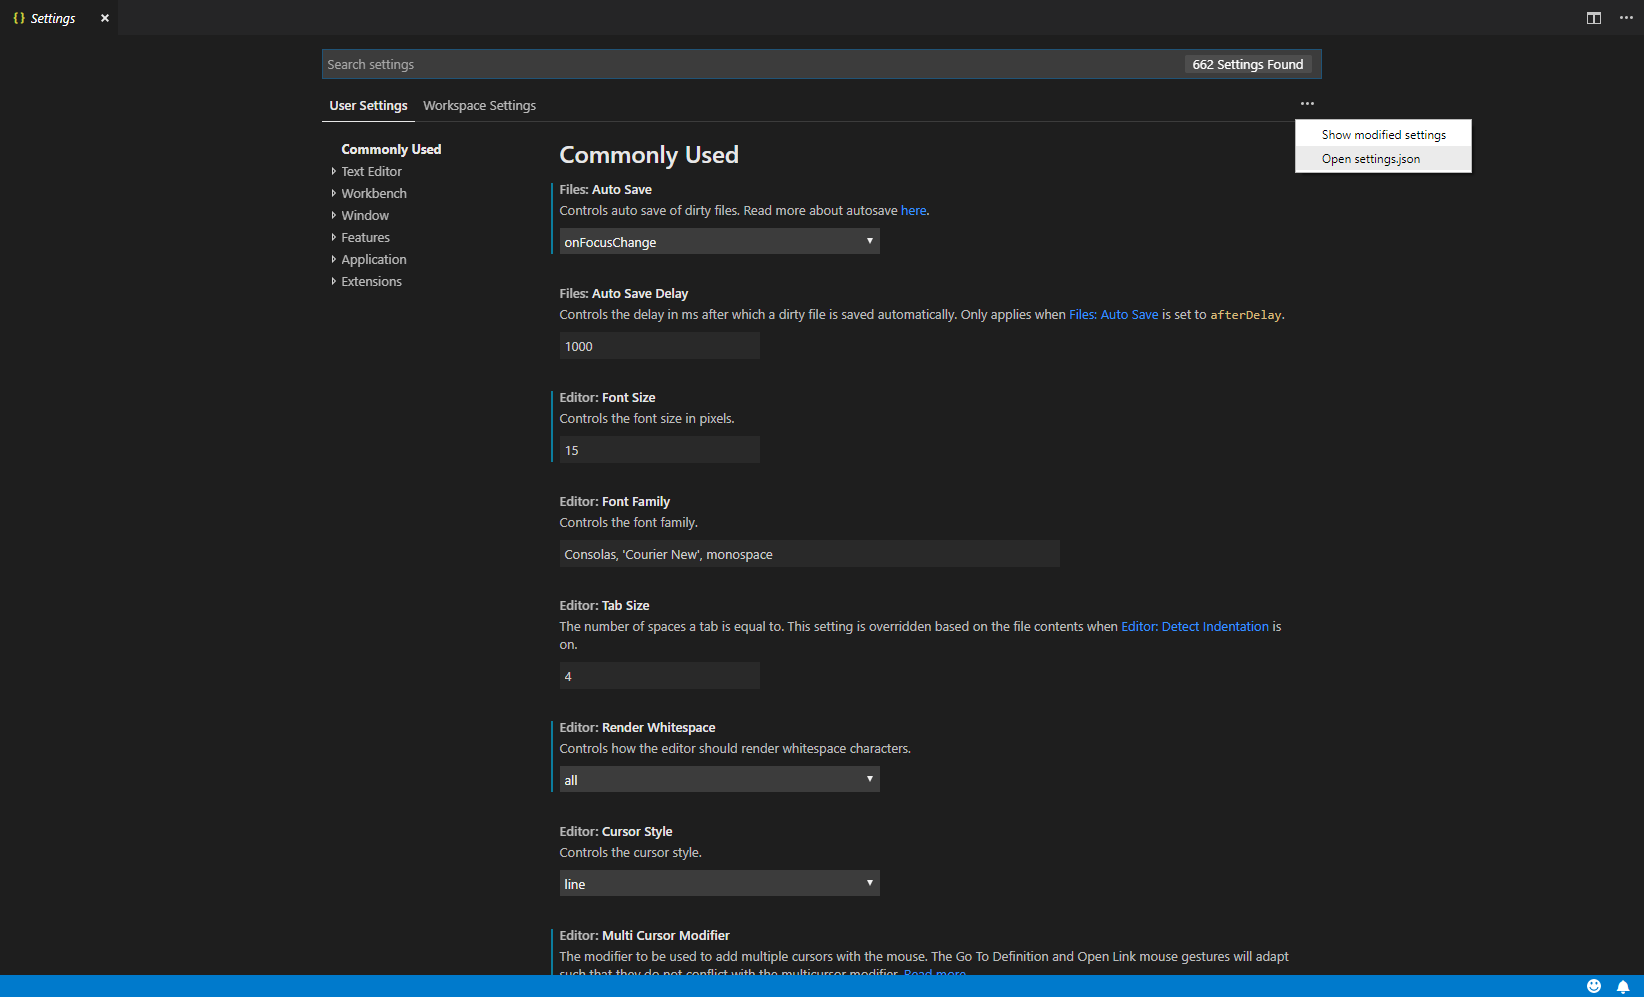
\includegraphics[width=\linewidth]{../resources/v1_27_settings.png}
	\caption{Getting to the old json based preview from the new settings menu}
	\label{fig:v1_27_settings}
\end{figure}


\section{Seperating Sources from Outputs} \label{sec:seperating_sources_from_outputs}
As a developer I manage everything that resembles code with version control, or more specificaly git.\\
One of the things that bothered me in the original configuration of \latex Workshop was that the folder containing my sources is repeatedly contaminated with the build products (and there are many of those). In addition to that, git recognizes these files, and writing gitignore rules for all of them is tedious and unaesthetic. For that reason I started searching for a way to redirect the build to a different directory.\\
On first glance I found the \textbf{latex-workshop.latex.outputDir} among the settings of \latex Workshop. This setting might seem appealing at first, but its function is different than expected. This setting lets the extension know where the build products are, rather than where to build them. Thanks to \href{https://github.com/James-Yu/LaTeX-Workshop/issues/548}{Oliver Clare's issue} on the \latex Workshop GitHub repository who investigated this issue as well, I was able to work around the problem.\\
In addition to changing \textbf{latex-workshop.latex.outputDir}, you must also edit the \textbf{latex-workshop.latex.tools} setting, that specifies the build command's arguments. By adding the arguments \texttt{-aux-directory=../<path>} and \texttt{-output-directory=../<path>} to each tool, we direct them to build the project in the directory \texttt{../<path>} right outside of our source folder.\\
Now the build folder can be easily added to the gitignore file, and problem solved! Figure \ref{fig:build_fix_settings} shows the fix with the path being \texttt{../build}.
\begin{figure}
	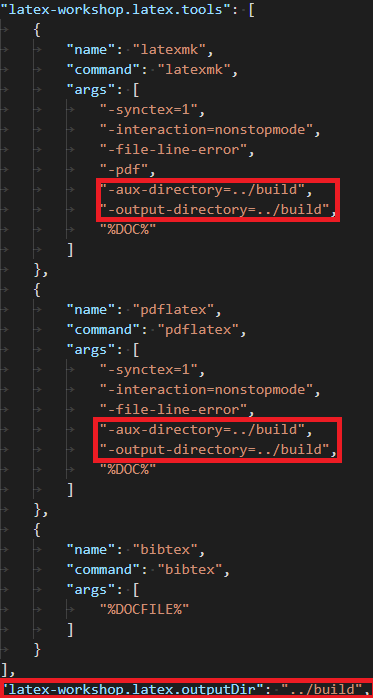
\includegraphics[scale=0.6,center]{../resources/build_fix_settings.png}
	\caption{The settings of \latex Workshop configured to build the project in \texttt{../build} folder}
	\label{fig:build_fix_settings}
\end{figure}

\end{document}